%!TEX root =  pulse_fitting_poster.tex
\begin{center}
  \begin{center} {\bf \Large \textsf {Photon Number Discrimination}}\end{center}
\end{center}

To determine the number of photodetection events, we calculate the signal area and assume that it is proportional to the energy absorbed~\cite{Cabrera2000509}.

To increase signal-to-noise ratio, we use the discriminator 
to identify integration windows surrounding pulses 
that exhibit a leading edge and decaying tail (Fig.1c).

In this way, pulses that are partially captured within our finite acquisition windows ($10~\mu$s) do not degrade the pulse-integral distinguishability between traces containing complete photodetection events.

We compute the pulse area $a$ for every trace
and organize them in histogram $C(a)$.

\begin{figurehere}
  \begin{center}
	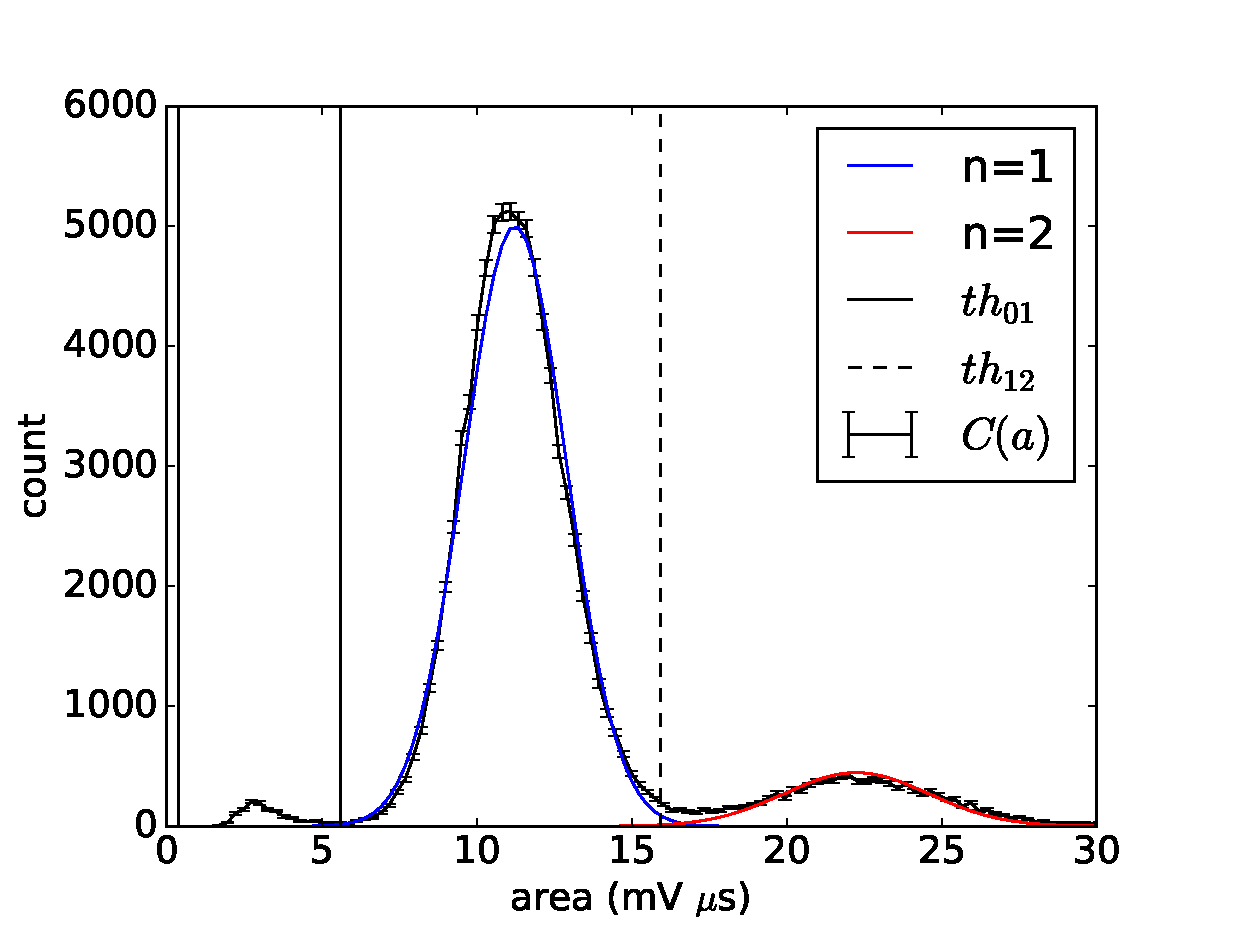
\includegraphics[width=0.9\linewidth]{figures/area_histogram_cw/area_histo_with_fit.eps}
  \end{center}
  % \vspace{-2cm}
  \figcaption{\label{fig:area_histos_comparison}
        Pulse area distribution $C(a)$ of the signal in the discriminated region.  
        The first bin ($a = 0$) corresponds to zero photodetection events being discriminated.
        The small distribution to the left of $th_{01} = 5.6$~mV$\,\mu$s corresponds to traces with detector noise exceeding $V_{th}$.
        The minimum of $C(a)$ between the $n=0$ and $n=1$ distribution corresponds to the threshold $th_{01}$.
        % Equally separated peaks corresponding to 1, 2, 3 and 4 photons demonstrates the linear dependence of the area with photon energy. 
        Error bars indicate Poissonian standard-deviation.
    }
 %    \figcaption{\label{fig:area_histos_comparison}
 %    The pulse area distribution obtained with the discriminator 
	% improves resolution: Red Line: area distribution of entire trace. Green line: area distribution of signal above $V_{th}$. Blue line: area distribution $C(a)$ of the signal region identified using the discriminator described in section~\ref{sec:disc}. Vertical lines: area thresholds $th_{mn}$ separating $m$ and $n$-photon events identified by the discriminator.
 %    }
\end{figurehere}
% \vspace{1cm}
We fit the area distribution 
identified by the discriminator 
corresponding to $n>0$ detection events 
to a linear combination of Gaussian distributions~
$G_1(a; a_1, \sigma_1)$ and $G_2(a; a_2, \sigma_2))$.

% \vspace{1cm}
% The ratio of the peak positions $a_2/a_1 = 1.98$ demonstrates the linear dependance of the pulse area with photon energy.

At the minimum overlap between the distributions $th_{12}$,
the probability of falsely identifying an $n=1$ trace as an $n=2$ trace is 0.2\%,
while
the probability of falsely identifying an $n=2$ trace as an $n=1$ trace is 0.3\%.
\vspace{1cm}
%
% We calibrate the detector by classifying a trace 
% with area $a \in [a_n-2\,\sigma_n,a_n+2\,\sigma_n]$ as an $n$-photon event.
%
% We determine the minimum overlap between $G_1(a; a_1, \sigma_1)$ and $G_2(a; a_2, \sigma_2)$ to be the threshold $th_{12}$. 
% At this threshold, 
% the probability of falsely identifying an $n=1$ trace as an $n=2$ trace is 0.2\%,
% while
% the probability of falsely identifying an $n=2$ trace as an $n=1$ trace is 0.3\%,